\documentclass[12pt,a4paper]{article}
\usepackage{times}
\usepackage{durhampaper}
\usepackage{harvard}
\usepackage{algorithm}
\usepackage{algpseudocode}
\usepackage{array}
\usepackage{graphicx}
\usepackage{subfig}
\usepackage{array}
\usepackage{titlesec}
\titlespacing{\section}{10pt}{3.25ex plus 1ex minus .2ex}{-\parskip}
\titlespacing{\subsection}{0pt}{3.25ex plus 1ex minus .2ex}{-\parskip}
\titlespacing{\figure}{0pt}{0}{-\parskip}
\newcolumntype{P}[1]{>{\centering\arraybackslash}p{#1}}
\graphicspath{ {images/}}

%remove spaces between references
\let\oldthebibliography\thebibliography
\let\endoldthebibliography\endthebibliography
\renewenvironment{thebibliography}[1]{
  \begin{oldthebibliography}{#1}
    \setlength{\itemsep}{0em}
    \setlength{\parskip}{0em}
}
{
  \end{oldthebibliography}
}

\citationmode{abbr}
\bibliographystyle{agsm}

\title{Investigation of Machine Learning Techniques for a Ball Balancing Task}
\author{Edward Hockedy}
\student{Edward Hockedy}
\supervisor{Dr. Magnus Bordewich}
\degree{MSc Computer Science}

\date{}

\begin{document}

\maketitle

\begin{abstract}
\subsection{Context}
Machine learning allows robots to learn behaviour when it is difficult to describe how to realise that behaviour. Balancing a ball on a tray is an example of such a task. Problems are that training can take a long time, or require human supervision. Simulation provides a way to speed up the training process. 

\subsection{Aims}
The main aim it to train a robot to keep a ball balanced on a tray by tilting the tray as the ball moves. Through this, the suitaiblity of different machine learning techniques for the task is explored. The project also looks at whether training in simulation can suitably speed up the training process.

\subsection{Solution}
The system comprises of a robot that holds a tray, observes the state of the ball, and tilts the tray. A simple 2D simulation of this was created. The machine learning techniques studied are Q-learning and neural networks. Refinements are made when training in an attempt to improve behaviour on the robot.

\subsection{Results}
The simulation-learnt behaviour is near perfect. When transferred to the robot, performance is adequate but not good. Refinements make performance no better. The level of performance on the robot is concluded to be mainly due to an insufficient number of possible actions, and capabilities of the robot.

\end{abstract}

\begin{keywords}
Reinforcement Learning, Robotics, Q-learning, Neural Networks, Simulation
\end{keywords}

\section{Introduction}
\subsection{Background}
Robotics is a rapidly advancing field with a wide range of applications. The primary aim of robots is to emulate and improve upon actions carried out by a human. Examples of uses include job automation, social care, dangerous environment exploration, entertainment, and more. One of the most difficult aspects of creating a working robot is programming how it will behave. In some cases it is sufficient to tell the robot exactly what it must do complete the task, and how to do it. In general, though, it is difficult to hard-code all actions a robot can take because there are many possibilities, with humans not knowing how to describe the optimal behaviour. Machine learning can help learn learn and generalise this behaviour.

There are two methods of machine learning studied and compared here - supervised learning and reinforcement learning. Supervised machine learning is the search for algorithms that reason from externally supplied instances to produce general hypotheses, which then make predictions about future instances \cite{sl}. This is equivalent to the robot observing a human complete the task. Reinforcement learning is the problem faced by an agent that must learn behaviour through trial-and-error interactions with a dynamic environment \cite{rl_survey}. The robot is told what a good state is to be in, and by trying out different actions the robot receives a reward or punishment dependent on the quality of the state it transitions to. Over repeated trials it updates its idea of what the optimal behaviour is to receive the most reward.

\subsection{Project Aim}
This project looks at different methods of machine learning to keep a ball on a tray, and explores techniques that can speed up the process and acheive better results. The final goal is to have a robot balance a ball on a tray by tiliting the tray. The learning process can take a long time with the robot, so a simulator is used to save time. The simulation is only a simple recreation of the ball and tray setup, so the project also investigates the suitability of using a simulation to learn real-world behaviour, and how well this behaviour transfers to the robot. 

The first machine learning method is Q-learning, a form of reinforcement learning. Q-learning makes learning agents interact with the environment, using the trial-and-error method to gather experience and train the action (decision) policy \cite{nao_balance}. Within the Q-learning study, two different styles of reward function are looked at. These are a simple reward based on only the new state, and a specific reward that uses information from the old state and new state. The second technique is a neural network, a massively parallel combination of simple processing unit which can acquire knowledge from environment through a learning process and store the knowledge in its connections \cite{nn_def}. The important difference between the techniques is that Q-learning lets the agent make actions for itself and learns based off a reward function which were good for a each state, whereas the neural network is explicitly old which actions are good to make in which state.

The refinement techniques used to try to improve performance were to add properties to the simulation to attempt to more closely model the real world setup. These additions were faster ball movment and a delay between actions. Experience replay was also investigated. Experience replay is where data acquired during the online learning process are stored and presented repeatedly to the underlying RL algorithm \cite{er}. This allows for the robot's actions to be reused in an attempt to mirror training on the actual robot.

\subsection{Outcomes}
For both Q-learning and the neural network, the behaviour learnt iin simulation was near perfect. When this behaviour was used for the robot, performance was not as good. It was concluded to be marginally better for the neural network. For the Q-learning rward function, the simple reward gave better final performance, but the specific reward learnt faster. The refinements added to the simulation did not help improve performance with the robot. 

\section{Related Work}
Machine learning is widely used for teaching behaviour to robots. \cite{nao_balance} uses Q-learning to teach a Nao robot to balance in certain poses that it cannot make before learning. The state space is of size 9. These states correspond to regions in the supporting area of the robot's feet. The action space is of size $7^5$. This gives over 150,000 state-action pairs. The reward function is relatively simple - the robot receives a positive reward if it stays stable after making an action, proportional to how stable it is. It receives a negative reward if it becomes unstable, with a large negative reward if it falls over. It was trained over 1000 episodes in simulation, where an episode was 100 movements, or until the robot fell. It was concluded that the robot successfully learnt to balance in the poses. A commonly studied task that is similar to the ball lanancing is cart-pole balancing. It requires a cart that can move left or right to keep a pole upright. An implementaion using Q-learning in \cite{cart_pole_webpage} use two bits of information to comprise a state. These were the angle of the pole and the angular velocity of the pole. The number of possible values were 6 and 3 respectively. There were two actions of move left or move right by a fixed amount. This was all done in a simulator, and the final training sequence took 136 episodes to learn. An an episode starts with the pole upright and runs until the pole falls past a certain angle. This gave a good idea of the size of state space that could be suitable. Interestingly, earlier tests shows that a larger state space took longer to train. \cite{real_pole} successfully completed the task for a real pole. It used an advanced form of Q-learning, but with a neural network instead of a Q-matrix as a function approximator. Training was done using experience replay. This eliminates the need to do repeated trials on the real pole.

Supervised learning is not commonly used in sophisticated robot behaviour learning. \cite{nn_then_dnn} uses a neural network trained in a supervised manner to create an initial reward approximation before performing reinforcement learning with a deep neural network. It was concluded that the pre-training helped the reinforcement learning converge faster. The tasks tested were the mountain-car problem, and a simulated autonomous wheeled robot.

Simulating the robot to decrease training times is common in literature. \cite{sim_robot_arm} investigates the task to grab a cube with a robotic arm after training in a simulation. The simulation closely models the robot arm. When the learnt behaviour was transferred to the real arm, the behaviour was closely followed until the point where the hand should have grabbed the cube, showing a not quite perfect behaviour recreation from simulation to real world despite a detailed simulation. \cite{arm_sim_door} also studied a robot arm, again with a sophisticated simulation. The tasks studied include reaching a random target, pulling a door, and moving an object. Discount factor was 0.98 and learn rate was a low value of 0.001 or 0.0001. Results show success when moving behaviour to the real world, but in some cases, it required a lot of training. \cite{nao_football} uses reinforcement learning to train a Nao robot to kick a football. The training takes place in a simulation package capable of simulating the behaviour of the entire robot, thus modelling the real world very closely. 

Experience replay is used commonly, as in \cite{air_hockey} where it is used to speed up training. This is necessary because the task of learning to score with an air hockey puck requires lots of trials and a simulator was not used. Another interesting point about this paper is its assumption that the best action to take is always hitting the puck at maximum speed. This is a reasonable assumption but brings up the question of the impact of making assumptions. It reduces the action-state space but could cause issues if the assumption is an incorrect one. Experience replay is successfully used by \cite{er} in conjunction with Q-learning for the tasks of keeping an inverted pendulum up, moving a robot arm, and a robot goal keeper. There are all tasks of a similar complexity to the ball balancing task. The paper concludes that experience replay performed well in simulation and real-world, and outperformed Q-learning. Experience replay is also addressed by \cite{er_deeper}. It highlights the fact that the amount of experience replay data can have a detrimental effect on performance, and that size of experience replay buffer should be chosen carefully even for simple tasks.

Overall, the surrounding literature shows the effectiveness of many of the techniques studied in this paper when tackling tasks of a similar complexity. For the Q-learning, the action state spaces ranged form very small \cite{cart_pole_webpage} to very large \cite{nao_balance}, showing it is very problem dependent on the complexity of the problem. Since the cart pole problem is most similar, the initial values for experimenting with state-action space size are based off this.

\section{Design}

\subsection{The Task}
The task is to balance a ball on a tray. The ball can move either to the left or the right. The goal for the robot is to keep the ball stable - in the middle of the tray with the velocity low. This is done by performing one of two actions, tilt the tray clockwise or tilt the tray anticlockwise. Only two actions were chosen to keep the number of options to a minimum, as more options would increase training time for the Q-learning. Three options were considered, with the third action being to not move, but it was decided that this option would be nullified by keeping the ball balanced by tilting between two angles repeatedly. At each step of the task the robot can observe information about the environment. This information comprises of the horizontal position of the ball with the origin at the centre, the horizontal velocity of the ball, and the angle of the tray. These pieces of information are continuous and must be mapped to discrete states. For example, the position of the ball is grouped into one of 12 possible positions on the tray. There are 12 velocity values, and 10 angle values. The combination of position, velocity and angle, makes up the current state of the environment. The task is to have the robot learn what the best action to take given any state. This is also important as it allows trays of different sizes to be used (provided the ball is the same size relatively), as it the case with the simulation and the robot. 

This task was chosen because it seemed simple enough to be achievable by a robot with the chosen learning techniques. The number of states is small, but big enough that it is hard to outright describe what to do in every scenario. It is also complex enough to be difficult to describe without mathematically modelling the whole system, but simple enough that the leant model can interpolate to unseen scenarios. The task is also achievable by humans when standing still, but becomes difficult when extra tasks are included such as walking. As such it is hoped that the robot could surpass human performance if it learns well enough. The task has obvious real-world applications. Whilst the level of performance achieved in this project is insufficient to have much real-world impact, a high level implementation of this behaviour could be used to carry object across a room, perhaps to an immobile patient, or to carry a person out of a dangerous environment.

\subsection{The Robot}
The robot used is the Nao from SoftBank robotics, shown in figures \ref{nao1} and \ref{nao2}. It is programmable with the API which gives control over the angles and position of joints. It has built in vision capabilities from the cameras located on its head. For the setup of this task, the robot is standing with its arms stretched out. It holds on to a cardboard tray flat in front of it. There is a small track that the ball sits in to prevent it from falling off the back or front of the tray, and two side buffers to prevent it from falling off the sides. The robot has built in functionality to track a red ball which is the tracking method used in this project. At any time the 3D position of the ball can be calculated by the robot. The velocity can then be obtained by observing the change in position over a given time period. The tray is tilted by the robot moving it arms. To determine the range of possible angles the robot can move between, the robot's arms were positioned by hand and the angles of the upper body joints were recorded. The angles were then manipulated so that the same angle could be recreate but in the opposite direction. The robot can then interpolate any angle between the maximum and minimum by taking a proportion of the maximum tilt and minimum tilt and adding the angles together.

The Nao was chosen over a purpose-built robot, for example one that consisted of just the tray and a single point of rotation. This is because the project was aimed to be as general as possible, as the methods used to learn behaviour for balancing will be more useful if the behaviour does not only work for a very specific instance. 

%\begin{figure}[H]
%	\centering
%	\includegraphics[width=10cm]{no_ball_front}
%	\caption{The Nao robot holding the tray in the horizontal position. There are two handles attached that it grabs onto with its hands.}
%	\label{nao1}
%\end{figure}
%\begin{figure}[H]
%	\centering
%	\includegraphics[width=10cm]{with_ball}
%	\caption{The Nao robot holding the tray with a ball. The head of the robot contains the camera moves as the ball moves.}
%	\label{nao2}
%\end{figure}

\begin{figure}[H]
\centering
\begin{minipage}[t]{.45\textwidth}
  \centering
  \includegraphics[width=1\linewidth]{no_ball_front}
  \caption{The Nao robot holding the tray in the horizontal position. There are two handles attached that it grabs onto with its hands.}
  \label{nao1}
\end{minipage}\quad
\begin{minipage}[t]{.45\textwidth}
  \centering
  \includegraphics[width=1\linewidth]{with_ball}
  \caption{The Nao robot holding the tray with a ball. The head of the robot contains the camera moves as the ball moves.}
  \label{nao2}
\end{minipage}
\end{figure}

\subsection{Simulation}
The simulated environment is two-dimensional and has a ball that rests on a tray that can tilt. The tray has barriers at either end to stop the ball from rolling off the ends. The tray can be tilted up to a maximum angle of 0.1 radians (5.7$^\circ$) in each direction. This simulation was built using the Pymunk physics engine. At each stage of the simulation the position and velocity of the ball can be directly read, as well as the angle of the tray.  Figure \ref{sim} shows the setup of the simulation.
\begin{figure}[H]
	\centering
	\includegraphics[width=10cm]{sim}
	\caption{The setup of the simulation}
	\label{sim}
\end{figure}

\subsection{Reinforcement Learning Approach}
The agent (robot/simulation) learns to balance the ball by trying actions and aiming to get a good reward. The method of reinforcement learning used is Q-learning. It is a model-free reinforcement learning technique, so there is no pre-learnt model the actions are based off. Over time, the agent learns the best action to take for each state. This information is stored in a Q-matrix, a matrix with a cell for each possible state. For each cell there is an array with a value for each action, with the value representing how good of an action it is given the current state. Learning works by the agent observing the state it is in, looking at the Q-matrix and finding the best action to take - the one with the greatest value. There is a probability that a different action will be taken instead - this allows for trialling different actions that may be better. It carries out the action and observes the state it ends up in. It receives a reward dependent on how good this new state is. The value for the action taken from the old state is then updated using the existing value, the reward, and the value of the best possible action to take given the new state. The intuition behind using the best value of the new state is that Q-learning assumes the agent is following an optimal policy for all future actions - the best possible chain of transitions between states, taking the optimal action each time. This is of course not the case during training, but over time it should converge to this. The update policy can be formalised as:
\[Q(s_t, a_t) = (1 - \alpha) \cdot Q(s_t, a_t) + \alpha\cdot(r_t + \gamma\cdot max Q(s_{t+1}, a)) \]
$s_t$ is the state at time t \\
$a_t$ is the action taken at time t \\
$r_t$ is the reward observed by taking $a_t$ from $s_t$\\
$\alpha$ is the learn rate. The higher this is the higher the updated value takes into account the reward and future state information compared with the existing value\\
$\gamma$ is the discount factor. The higher this is, the more important future values are taken to be. A small value only looks at the immediate future of transitions\\

For the implementation of Q-learning in this project, the reward was determined in two ways. The first was with a very specific reward, based on what a human would intuitively think is the best action to take at each step. It used both the current state information and previous state information. The reward is decided based on the criteria outlined in algorithm \ref{ql_specific}.
\begin{algorithm}[H]
	\caption{Calculate reward using very specific criteria}
	\label{ql_specific}
	\begin{algorithmic}[1]
		\State $reward = 0$
		\If {$current\_velocity > 0$ \textbf{AND} $current\_angle > previous\_angle$}
			\State $reward = 1 - |\frac{current\_position}{tray\_width}|$
		\ElsIf {$current\_velocity < 0$ \textbf{AND} $current\_angle < previous\_angle$}
			\State $reward = 1 - |\frac{current\_position}{tray\_width}|$
		\ElsIf {$|current\_velocity| < max\_velocity*0.01$ \textbf{AND} $|current\_position| < |previous\_position|$}
			\State $reward = 1 - |\frac{current\_position}{tray\_width}|$
		\Else 
			\State $reward = -1 * (1 -|\frac{current\_position}{tray\_width}|)$
		\EndIf
	\end{algorithmic}
\end{algorithm}
Algorithm \ref{ql_specific} gives a positive reward if the ball has a positive velocity (left to right) and the tray has moved anticlockwise, effectively slowing it down, and vice-versa on line 4. It also gives a positive reward if the ball is at the very low speed of 1\% of the maximum speed and moving towards the centre of the tray. Since the tray is centred on 0, the magnitude of the position determines how close to the centre the ball is, with a smaller magnitude meaning the ball is closer. If none of these cases are matched, then a negative reward is given. In each case of the reward, the size is determined by how far the ball is to the centre, with a bigger reward being given if the ball is closer to the centre.

The second reward scheme is much simpler, using only the current state information to specify the states that deserve a good reward, with everything else getting a negative reward. The reward scheme is outlines in algorithm \ref{ql_general}.

\begin{algorithm}[H]
	\caption{Calculate reward using very general criteria}
	\label{ql_general}
	\begin{algorithmic}[1]
		\State $reward = 0$
		\State$pos\_range$ = length of tray * 0.2
		\State$vel\_range$ = maximum velocity * 0.2
		\If {$- pos\_range< pos < pos\_range$
			\textbf{AND}
			 $-vel\_range < vel < vel\_range$}
			\State $reward = 1$
		\Else 
			\State $reward = -1$
		\EndIf
	\end{algorithmic}
\end{algorithm}
Algorithm \ref{ql_general} gives a positive reward if the ball is in one of the segments determined to be good. The $pos\_range$ and $vel\_range$ variables determine the range of ball positions and velocities that are considered good. Maximum velocity is the maximum velocity the ball can reach by letting it roll from one end to the other at maximum angle.

The training begins with the ball in a random position and the tray at a random angle. At each step the agent chooses the action it thinks is the best for the given state. No prior knowledge is given for Q-learning, so all table values are 0. To assign values, at the start there is a very high probability of taking a random action. This probability is known as the exploration rate. This allows the agent to build up some scores for different states. Over time the Q-matrix fills up and the values start to converge. The explore rate decreases over time to allow the agent to start taking the best actions. Most states will have been sampled after enough time, so exploration is not needed. The Q-matrix should end up with the states all suitably sampled, and the rewards should have propagated through via the update function such that a distribution of state quality exists through the matrix.

\subsection{Supervised Learning Approach}
The first step in the supervised learning approach was to generate the training data. A ball is placed on the tray at a random angle, and a user could press keys to turn the tray one angle segment clockwise or anticlockwise, depending on what was required to keep the ball balanced. At each key press, the state and action taken was recorded. This was repeated over many iterations to build up a reasonably sized data set that covered many situations. About 360 items of training data were recorded.
%A neural network is a way to theoretically simulate any function, by combining many simple, linearly-separable functions known as neurons. The neurons e
%exist in layers with one input layer and one output layer. Between the layers exists weights from each neuron to each neuron in the next layer. The network is trained by passing through the input data. Each neuron receives some input from the previous layer, maps the combination of input values to an output value depending on its function, then outputs a value that goes to the next layer. Once the input data has passed through the network, the output from the network is compared with the actual output from the training data. The difference is calculated, and that error is used to refine the weights between the neurons. As more data is passed through, the network gets refined and begins to learn which inputs lead to which outputs.

The network input layer has three nodes for position segment, velocity segment and angle segment. The output is one of the two possible actions - tilt left or tilt right. The rest of the structure of the network was determined by experimentation. It was thought that a small network would suffice since the problem is quite simple, and the function that the network would approximate is relatively smooth i.e. there are distinct groups of similar states that give the same output, and changing state by a small amount does often not affect the output. The values tested ranged from 2 to 10 nodes per layer, for one and two layers. 

\subsection{From Simulation To Robot}
Difficulties arose when using learnt behaviour with the robot. They are discussed here. The biggest issue was that the arms of the robot overheated quickly. For safety reasons the overheated joint loses stiffness, meaning the joint cannot be moved against gravity. This usually happened about ten minutes after having the robot move its arms frequently. This was not a huge issue in the long run because the focus was to do all training in simulation, but any training or data collection that happened on the robot because difficult and time consuming when waiting for the robot to cool down. To circumvent this, two robots were used so one could cool down whilst the other was used. This issue highlights the usefulness of simulation in robot movement training.

Another issue was the accuracy of the ball tracking. The accuracy of the tracking functio was quite low, and the computed position value of the ball could vary slightly despite the ball not moving. The built-in tracking function was continuously called by a thread running in the background. The frequency of update caused issues since a more frequent update meant the changes in position were small, so the relative error in position detection was greater. Too infrequent updates limited the number of actions the robot could take.

The change of angle function calls to the robot joints are non-blocking. This means that as soon as an update to a joint is called, another one can be made. As such, it can limit the robot's ability to quickly switch between two angles, something that occurs quite often when balancing. Instead, the robot will stick to a single angle for a while when it should be changing, then update a few angles at a time. 

% An issue arose when choosing the frequency of updating the ball information however. Too frequent updates meant the values may not update, and as such the velocity value would be zero which is often not the case. Too infrequent updates could mean that the robot is limited in the number of actions it can perform, since there must be a change in state otherwise an action is taken twice in a row. Since actions are limited by ball readings, if there are too few it means there may not be enough actions take in order for the tray to move the required amount to keep the ball balanced. Since the tray must move through the states one by one, if the updates are too slow then the ball may have moved past before any meaningful movement can occur. The accuracy of the method as a whole is also not perfect, and position value can vary quite a bit even for cases where the ball does not change position. Less frequent updates mean the error has less impact, but again less frequent updates can lead to issues.

\subsection{Refining Simulation}
The robot did not successfully emulate the simulation to the desired quality. From observing this behaviour, it was seen that there are only about 5 actions taken from the ball travelling from one end of the tray to the other. More actions were required to fully rotate the tray to a meaningful angle, and so the current state of the Q-matrix was not sufficient. In particular, if the robot took an action that was not optimal because the Q-matrix was insufficiently trained, then it could cause the ball to roll away. There are some states where the difference in value for each action was minimal, since each action gave the same reward. The only disparity came from which action was taken most recently, as this will have had the most recent value update. The simulation was changed to closer reflect the robot's mechanics, with the hope of learning to deal with the difficulties presented by the robot. To do this, a delay was added between actions in the simulation. It was hoped that this would allow the agent to learn to deal with less frequent actions. The speed of the ball was also increased since the real ball moves faster.

%To help with the non-optimal action being chosen, a "Q-matrix consensus" was taken when choosing an action. This takes into account the best action for the current state, but also the best actions for the states with a velocity segment difference of one either side, and the states with a position segment different either side. Assuming the current state does not involve the maximum or minimum velocity or position, this gives five votes for what the best action to take is. The action with the highest number of votes is taken. In the result of a tie, the original action is taken. The intuition behind this is that the states considered are similar to the current state, so will most likely have similar optimal actions. So in the case that the current state's values have not converged in the Q-matrix, it is hoped that some of the others have, leading to a better estimation of what the optimal state is. MAYBE REMOVE THIS

%After seeing how the simulated behaviour worked with the robot, the simulation was changed to reflect the robots mechanics more closely with the hope of learning to deal with the difficulties present in the robot. The two behaviours incorporated into the robot are the delay between actions, and the overall speed of the ball. The delay between actions helps model the speed of the robot updating of the tray angle, which is slower then the simulation. After the tray has moved, it waits a set number of frames before deciding on the new action to perform. The speed of the ball is reflected in the simulation by increasing the number of steps taken per frame of the simulation. 

%After training in the simulation for the same number of iterations of the original simulation, performance was definitely worse. However, this was not unexpected. Unfortunately, performance on the robot showed little improvement. 

\subsection{Experience Replay}
A dataset of actions taken by the robot was recorded. By using this data with the Q-learning algorithm, behaviour is learnt from the robot’s own actions instead of simulated actions. This makes the actions the most accurate representation of what the robot would do. An experience comprises of an initial state, the action taken by the robot (not necessarily the one it believes to be optimal), the state it ends up in, and the reward received. Experience replay uses a Q-matrix trained in simulation as the Q-matrix for the update function. To train in this way, an experience is randomly chosen. Then, the new Q-matrix is updated for that state and action using the recorded reward and the future state value taken from the pre-trained Q-matrix. The pre-trained matrix is used since this has learnt what the best actions to take are. This emulates the robot performing the action and then taking the optimal next choices. 

This data was recorded by having the Nao hold the tray and carry out actions. It was told to do a combination of random actions or follow a learnt behaviour to allow it to experience as many states as possible. For each possible state, a maximum of 20 actions and next states were recorded. Multiple states were recorded since the next state could vary quite a lot. Not all states had 20 experiences recorded. In total, about 5900 experiences were recorded, for a total of 1440 states. Some states had no experiences recoded, as they were never experienced when gathering the data. This is okay because they are unlikely to be experienced in actual balancing. 

%Unfortunately, once again the improvement was not significant, but perhaps marginally better. The most interesting observation was that the simulation, when ran after experience replay, mimicked the behaviour of the robot quite closely - the ball was rolled from end to end. This shows that the simulation was capable of learning the robot's behaviour, but not the other way around. MOVE TO RESULTS?

\section{Results}
The success of learnt behaviour for this task cannot be quantified as there is no end state. Instead, the ball position over time is observed and used to assess quality of learnt behaviour. If after training the ball is stuck at one end, or moves between the two, then it is not balanced. If it stays around the middle, it is balanced. For each training run, the position at each step of the simulation was recorded. This information can be plotted on a graph showing the motion of the ball over time, and is the metric used here to assess performance. 

The results presented here show the performance of the each method. This includes training in the simulation and performance on the robot. Also shown is refinement of parameters and any optimisations made to get to the best performance of the method. 

\subsection{Q-learning Parameter Refinement}
The first stage towards best performance for Q-learning was to find the parameters that converged the Q-matrix fastest.
\begin{table}[htb]
\centering
\caption{Q-learning parameters}
\vspace*{6pt}
\label{q_params}
\begin{tabular}{>{\raggedright}p{0.2\linewidth}p{0.55\linewidth}p{0.17\linewidth}}\hline
Parameter & Description& Tested Values\\ \hline\hline
Initial exploration rate & The starting probability of taking a different action to the one though to be the optimal & 0.2, 0.5, 1\\ \hline
Exploration rate reduction frequency & The number of times the exploration rate is reduced & 5, 10, 20\\ \hline
Exploration rate reduction value & The percentage to reduce the exploration rate by & 10, 20, 33.3, 50 \\\hline
Learn rate & The proportion the updated value in the Q-matrix is made up from learnt information compared to existing information & 0.1, 0.4, 0.5,  0.7 \\\hline
Discount factor & The influence future rewards have on updating the value for the current state and action & 0.5, 0.8, 0.9, 0.99 \\\hline
\end{tabular}
\end{table}
To do this, various grid searchs were done to find the best combination of parameters. Many of the parameters are dependent on each other, so it was important to test all combinations of different values. The following tests in simulation were run for 50000 iterations, where an iteration is an action.

The parameters that affect the exploration rate are not independent, so all combinations of their values were tested. The quality of each combination was judged by analysing the position of the ball over 5000 iterations, with explore rate set to 0. The best combination of parameters is shown in figure \ref{f3}. An initial exploration rate of 0.5 makes sense, since at the start there is no optimal action for any state - each action has an initial value of 0, so the first action is chosen by default. Having an exploration rate of 0.5 means half the time that action will be taken, and the other half of the time the other action will be taken. This is a good way to get a sample of actions through the matrix. The combination of reduction value multiplier 1.5 and reduction frequency 20 allows for sufficient exploration whilst training but diminishes quick enough to not cause random actions when the best actions have already been found. Figure \ref{f1} shows the performance of the trained Q-matrix with these parameters over the 5000 time frames.

\begin{figure}[H]
	\centering
	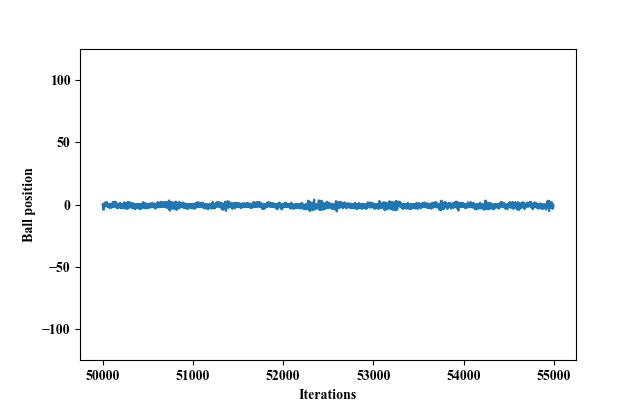
\includegraphics[width=10cm]{100_small}
	\caption{The position of the ball over 5000 actions. Note that the width of the tray is 125 in each direction, so the ball stays very confortably in the centre}
	\label{f1}
\end{figure}
\begin{figure}[H]
	\centering
	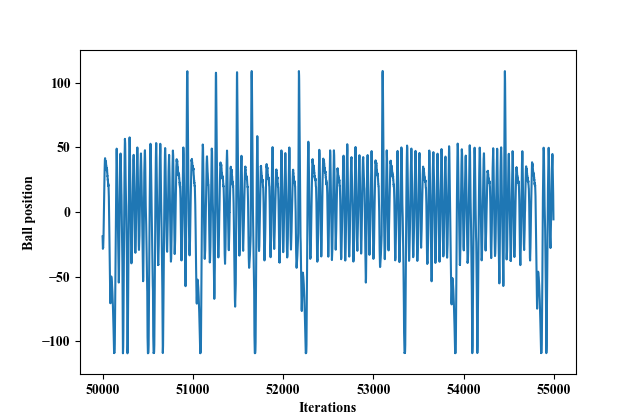
\includegraphics[width=10cm]{101_small}
	\caption{An example of learnt behaviour that was unsuccessful. Initial exploration rate was 0.2, reduction value was 1.5, number of reductions was 5. The repetition of the pattern shows that it has slightly learnt the ability to balance, however the amplitude is large.}
	\label{f2}
\end{figure}
%Sims 88 to 115 compares exploration rate stuff
% After 1st round of tests, 100 was best. This is erv:1.5, init:0.5, num:20. About 30000 iterations to converge
%\subsubsection{Initial exploration rate}

For learn rate and discount factor, low values of both gave poor results. For higher values difference in performance was negligible. Repeated tests decided the best values were a learn rate of 0.4 and a discount factor of 0.9. These results make sense. The learn rate is just below half, showing that the new information is important to the updating process, but is just a bit less important than the existing data. Anything higher could drown out the existing value stored, and since there is quite a lot of exploration, especially early on, it is important to not let the agent change its values too hastily. The discount factor is high since future actions are important in this task. If not, it would send the ball to the centre of the tray as quick as possible, whether sometimes it is better to move it gradually to avoid overshooting. A possible reason 0.9 was superior to 0.99 (if only marginally) is that it is sometimes important to focus on the very short term, for instance when right at the edge of the tray - it is better to move the ball away quickly than roll off.

Convergence speed is another important aspect to learning. In a small task like this training takes less than a minute. For a larger task however, it is important to reach the desired performance level as soon as possible. It is hard to know when the task is fully learnt since there is no exact completion criteria. However, looking at the plot of position against time for the whole learning procedure can show when the ball is kept in a constant position. Figure \ref{f3} shows this for the agent learning over 50000 iterations with the refined parameters.
\begin{figure}[H]
	\centering
	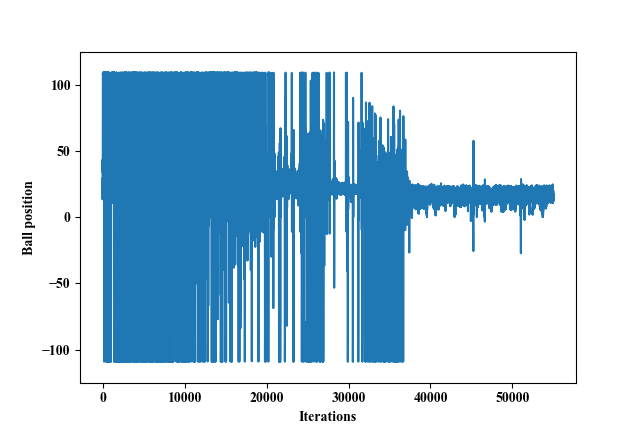
\includegraphics[width=10cm]{153_small}
	\caption{The position of the ball over an entire training session. At the start the ball rapidly rolls between either side of the tray. Over time this becomes less frequent as behaviour to prevent this is learnt, and the random actions happen less frequently. By the end of the training, the ball is kept in the middle of the tray.}
	\label{f3}
\end{figure}
Figure \ref{f3} shows that convergence happens around 30000 time steps. Despite this, it is not sufficient to cut off training at 30000 iterations. Since exploration rate is linked to the number of iterations, with the same initial parameters the learning would be different. Additionally, it is probably best to continue learning to solidify behaviour. 

Table \ref{q_params} shows the values that gave the best performance for Q-learning. They may not be optimal, but testing suggests they will be close and any improvements will be minor. The focus of the project is not to find the absolute best parameters for the task, so these values will suffice as they give a suitable Q-matrix convergence speed.
\begin{table}[htb]
\centering
\caption{Final Q-learning parameters}

\label{q_params}
\begin{tabular}{>{\raggedright}p{0.4\linewidth}p{0.2\linewidth}}\hline
Parameter & Refined Value\\ \hline\hline
Initial exploration rate & 0.5\\ \hline
Exploration rate reduction frequency & 20\\ \hline
Exploration rate reduction value & 33.3\% \\\hline
Learn rate & 0.4 \\\hline
Discount factor & 0.9 \\\hline
\end{tabular}
\end{table}


\subsection{General Reward vs Specific Reward for Q-learning in Simulation}
\begin{figure}[H]
	\centering
	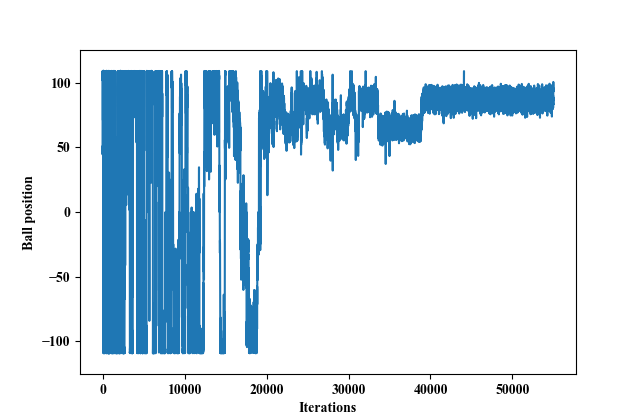
\includegraphics[width=10cm]{157}
	\caption{The position of the ball when training with a detailed reward function.}
	\label{f5}
\end{figure}
For the parameter tuning, the reward used was the general reward. Figure \ref{f5} shows the performance of the trainer as it learns with the specific reward function over 50000 iterations. It converges faster than the general reward - convergence happens after about 20000 steps. However, the position of the ball is off centre. This could be considered balanced, but to give the best chance of keeping balanced in the case of sudden movement, a central position is preferred. A specific reward likely gives this result as it aims to bring the ball to a stop as soon as possible and acts to counteract any movement that may accelerate the ball. As such, it gets stuck wherever it is and never allows the ball to accelerate even a small amount to the centre of the tray since there is no consideration of future actions, except for the case where velocity is below 1\% of the maximum velocity.

\subsection{Neural Network in Simulation}
To find the best neural network with the shortest training time, the parameters shown in table \ref{nn_params} were tested. The structure format is given as the number of neurons for each layer, so (x, y) has x neurons in the first layer and y neurons in the second layer. The number of epochs is the number of times the trainer goes through the entire data set. Results showed that all combinations except for the (2) structure (single layer with two neurons) and 50 training epochs worked sufficiently. By comparing the graphs of the ball position over time for the trained network, as well as the time to train, the best structure was decided to be (2, 2). Other structures worked similarly well but the smaller structure meant shorter training time and less chance of overfitting. The decided number of epochs was 100 as it was enough to train sufficiently, did not take too long, and is less prone to overfitting then more epochs. Figure \ref{nn_param_test} shows the position over time for the trained network of chosen size. It balances the ball very well.
%from about 60 to 92 are the tests for nn params
\begin{table}[htb]
\centering
\caption{Neural network parameters. The best structure was (2, 2), best number of epochs was 100.}
\label{nn_params}
\begin{tabular}{>{\raggedright}p{0.3\linewidth}p{0.4\linewidth}}\hline
Parameter & Tested values\\ \hline\hline
Hidden layers structure & (2), (5), (10), (2, 2), (5, 5), (10, 10)\\ \hline
Number of training epochs & 50, 100, 150, 200\\ \hline
\end{tabular}
\end{table}
\begin{figure}[H]
	\centering
	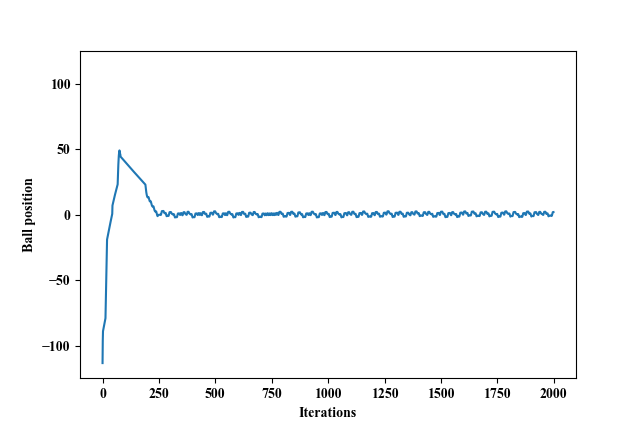
\includegraphics[width=10cm]{86_nn}
	\caption{The position of the ball in simulation or 2000 time steps for the trained neural network. The ball starts at the side and is moved closer to the centre. It overshoots the centre at first but is moved back and stays in the middle for the remainder of the time.}
	\label{nn_param_test}
\end{figure}

\subsection{General Reward Q-learning with Robot}
Performance was worse on the robot than in simulation. As seen in figure \ref{q_nao}, the ball hits the sides of the tray numerous times. There are some instances of getting the ball under control when it is in the middle of the tray, as seen by the changes of direction around the centre of the y-axis.
\begin{figure}[H]
	\centering
    \subfloat[Instance 1]{{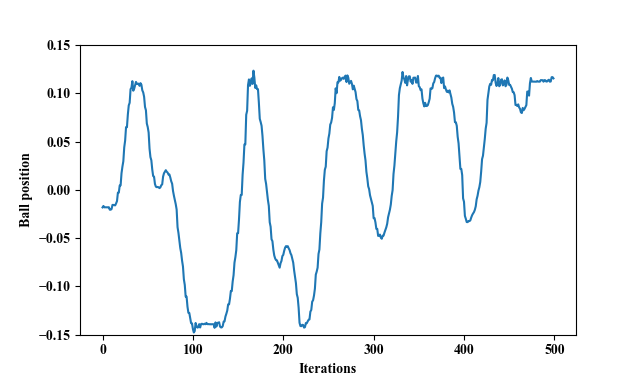
\includegraphics[width=8.5cm]{0_nao_q} }}%
    \subfloat[Instance 2]{{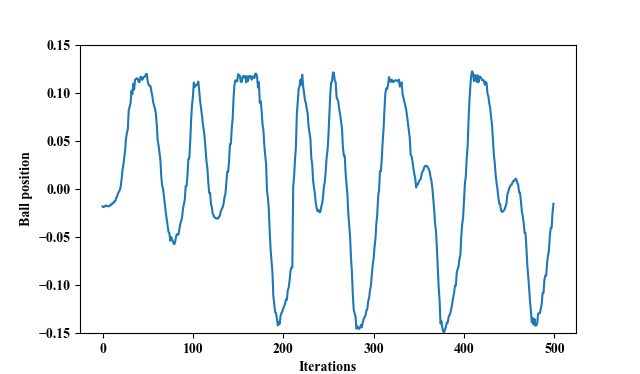
\includegraphics[width=8.5cm]{1_nao_q} }}%
	\caption{Two instances of the ball balancing on the tray with the robot in control. Actions are decided by the trained Q-matrix. Two different cases were shown since performance on the robot could vary quite a lot.}
	\label{q_nao}
\end{figure}

\subsection{Specific Reward Q-learning with Robot}
The specific reward function did not fare much better than the general reward function when learnt behaviour was transferred to the robot. Interestingly, it does mirror the simulated behaviour in that it tends to keep the ball to one side of the tray and counters the movement when the ball tries to move back into the centre.
\begin{figure}[H]
	\centering
    \subfloat[Instance 1]{{\includegraphics[width=8.5cm]{2_nao_specific} }}%
    \subfloat[Instance 2]{{\includegraphics[width=8.5cm]{32_nao_specific} }}%
	\caption{Two instances of the ball balancing on the tray with the robot in control and the detailed reward function. The behaviour is very reactive to the ball speeding up towards the centre and tends to keep the ball to one side.}
	\label{q_nao_specific}
\end{figure}

\subsection{Neural Network with Robot}
Performance of the balancing behaviour on the robot was worse than in simulation. The performance was not bad enough to be considered a failure however. Figure \ref{nn_nao} shows the ball position changing over time on the robot. In both cases it does touch the end a few times, but the behaviour does mirror the behaviour in simulation. That is, as the ball approaches the end of the tray, the tray tilts to oppose the movement and the ball rolls in the opposite direction. most of the changes in direction keep the ball away from the sides of the tray. This is evident from the changes of direction in both graphs in figure \ref{nn_nao}.
\begin{figure}[H]
	\centering
    \subfloat[Instance 1]{{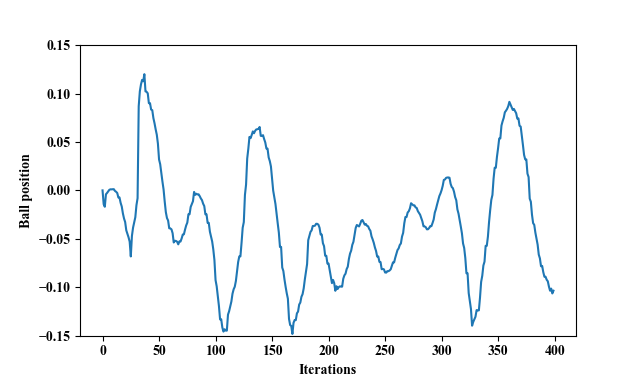
\includegraphics[width=8.5cm]{8_nn_nao} }}%
    \subfloat[Instance 2]{{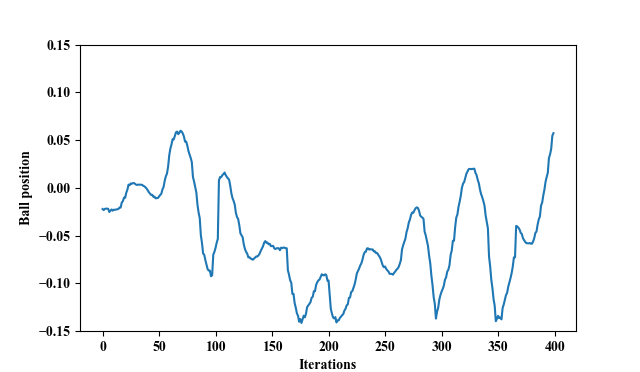
\includegraphics[width=8.5cm]{9_nn_nao} }}%
	\caption{Two instances of the ball balancing on the tray with the robot in control. Actions are decided by the trained neural network. Two different cases were shown since performance on the robot could vary quite a lot.}
	\label{nn_nao}
\end{figure}
\subsection{Refined Q-learning in Simulation}
The first refinement technique to be tested was the inclusion of a delay between actions, and an increase in the speed of the ball in the simulation. The delayed actions help mimic the robot because the robot can take actions less frequently than the simulation. This is because of the time taken for the robot to execute an action, as well as the frequency of obtaining state information. The increased ball speed in the simulation more accurately represents the speed of the ball in the real world. The original variance in ball speed between robot and simulation could be down to a range of factors including friction between the ball and tray and weight of the ball.

The same parameter refinement as the original simulation was carried out in case the results differed. It was found that most of the best parameters from the original simulation were still the best parameters. The only difference was exploration rate reduction value, where a value of 50\% reduction was found to be marginally better than 33\%, but only by observation of the graphs after the few tests run for each set of parameters. The difference in performance was minimal.

The overall performance of the learnt model was worse with the delay and ball speed up. It did still perform to a level that could be considered balancing and did not touch the end of the tray very often. Figure \ref{refined_sim_general} shows the behaviour after 50000 iterations. This decrease in performance is not unsurprising since the tray can adjust less frequently so has fewer chances to counteract the movement of the ball. The increased speed of the ball also means any movement the ball makes will cover more distance and it will hit the sides quicker.

\begin{figure}[H]
	\centering
	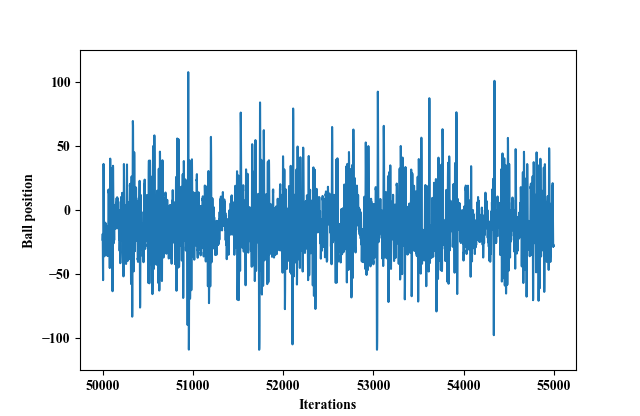
\includegraphics[width=10cm]{195}
	\caption{The position of the ball when training with the delay and increased ball speed. The ball rolls to the edges a few times over the 5000 time steps, but the tray gets it under control again. }
	\label{refined_sim_general}
\end{figure}

%Doing just ER by itself could lead to the ball becoming stuck. This is due to differnces between the physics of the simulation and the robot. SInce the behaviour is learnt purely from the experiences on the actual robot, the accuracy of the simulation to the robot was irrelevant for training, so this issue only arises when viewing the leanrt behaviour in simulation. When plotting the change of Q-values over time, it can be seen that the values chosen here converge. However, the action that is optimal can change for some pairs of actions. This shows that both actions are essentually equal in their quality. THis means that the one that is considered best can change over time, and the time that the training is stopped determines which is optimal. Since The action with the highest value is outright chosen each time, the other action which is equally as good may not be. Of course in many cases it is not the case that both ations are equally good. in fact in a task like this there is almost always a superior action. In the cases that the wrong action is learnt to be optimal however, it can have a big impact such as the ball getting stuck. As a solution to this, an alternative action selection process was implemented. Instead of picking the action with the highest value, there is a chance of picking either action that is proportional to the values of the actions. For each action, its value as a proportion of the sum of all values is found, and this is the chance that actuion is chosen. This means if two actions have very similar values, then they are equally likely to be chosen. This is only applied if both actions have positive values or both have negative values. In the case where one action is positive and one is negative, then the choice is clear. Frm running the simulations again using the behaviour learnt from experienc replay, the performance is better. The ballno longer gets stuck at one side, however the overall performance is poor. THis is most likely due to the randomness that is now in the action selection process. As such, this proportional action selection can be considered a trade-off between optimal performance and average performance - if training goes well such that the close-valued actions end up with the optimal action having the higher value, then the performance will be wore. In the case that the non-optimal behaviour is learnt, then the proportional actin slectin prevents any destructive behaviour. The behaviour seen is not good enough to be considered balancing. The behaviour generally tilts the ball from one end to the other, indicating at some learnt behaviour - enough to get the ball away from the immediate edge - but not enough to keep it centered. 

%WHY DO ER QVALS CONVERGE TO VALUES BUT NORMAL SIM QVALS DONT - Think this is because there are quite a few cells that are at 0 since no data exists for those cells. This means the 2nd half of the update function can often be low, which is what keeps the q-val bounded. I THINK WE JUST NEED EVEN MORE ER DATA :/

%Some cells were 0 because the states were not recorded in the er data

%Say used specific reward on nao as it was better than general in simulation.

%The behaviour learnt with delay definitely converges since we can view the entire graph of ball position as learning goes on. sim_q 340 shows this behaviour.
\subsection{Refined Q-learning with Robot}
Figure \ref{delay_noer_1} shows the performance of the robot with behaviour learnt from the simulation with added delay. Performance was not noticeably better than the behaviour learnt without the delay. 
\begin{figure}[H]
	\centering
    \subfloat[Instance 1]{{\includegraphics[width=8.5cm]{43_delay} }}%
    \subfloat[Instance 2]{{\includegraphics[width=8.5cm]{44_delay} }}%
	\caption{Two instances of the Nao balancing the ball using behaviour learnt from the simulation with a delay.}
	\label{delay_noer_1}
\end{figure}

The experience replay did not improve the results either. As shown by figure \ref{er_nao}, performance is not what would be considered to be balancing the ball. It does appear to have the general behaviour of changing the direction of the ball as it speeds up, however. 
\begin{figure}[H]
	\centering
    \subfloat[Instance 1]{{\includegraphics[width=8.5cm]{36_er} }}%
    \subfloat[Instance 2]{{\includegraphics[width=8.5cm]{37_er} }}%
	\caption{Two instances of the Nao balancing the ball using behaviour learnt from the Q-matrix trained using experience replay, using a Q-matrix trained in simulation to get the future rewards in the update function.}
	\label{er_nao}
\end{figure}

\section{Evaluation}
\subsection{Supervised Learning vs Reinforcement Learning}
In supervised learning the agent is told what a good action is to take in a given state. This is not necessarily bad for behaviour learning and works well because the ball balancing task is simple. However, in general it might not be suitable for a more complex task, since it is almost impossible to fully describe exactly how an agent should behave. Another downside to this technique is that it requires generation of training data from human input. This means in this case the agent can only do as well as the human can. 
This technique is useful because it allows for interpolation between states, which means it deals well with unseen circumstances. The neural network always gives an output no matter what, and assuming it has seen some somewhat similar cases it should give a decent output. In contrast, the Q-matrix may have some blank cells that have never been explored before, meaning there is no way to infer what a good action to take would be. Training time and data size are also an advantage with the neural network. The Q-matrix must store data for every single state, and since a state is a 3-dimensional vector, the state space grows fast, which means training takes a long time too. The neural network will not be close to the size of the Q-matrix, even if there are many neurons. The training data may be quite large, but once the model is trained it is not required. 
From the results, it is concluded that the supervised learning approach was better suited to the ball balancing task than the reinforcement learning approach. 

\subsection{Failure of Refinement Process}
Adding delay to the simulation didn't improve the results, nor did it make them much worse. This is likely because the Q-matrix learnt in simulation will be the same as without the delay. This is because the fundamental behaviour is the same regardless of whether there is a delay. For each state, out of the two possible actions to take, there is always an optimal one that will help to slow the ball down and keep it closer to the centre. The delay will not really affect which is the best action to take.

The ineffectiveness of experience replay can be explained with an example shown in table \ref{er_example}. This shows the 18 experiences recorded for the state (8, 4, 6), the action taken, the resultant state, and the reward for being in that new state. Some new states are entered more than once, as shown by frequency. This state was chosen as it is reasonably common with many outcomes with different rewards. This wide variety of outcomes was the main issue with the experience replay. Since there are so many outcomes, it shows that the robot is imprecise with the actions it makes, and the ball can end up in a wide variety of places for the same action. This happens for a number of reasons. Firstly, because the values of speed and velocity have been mapped to discrete segments, it means that similar values have been grouped together. As such, two positions could be at the opposite ends of the segment, and as such would have quite different values. Secondly, the inaccuracy in the Nao's ball tracking measurements introduces variation in the measured states. Lastly, the real world has so many possibilities of things that could happen, then it is not unreasonable that the ball behaves so differently each time. Because of this variation, it was not uncommon for the same action  to have outcomes with differing rewards. Table \ref{er_example} shows this is the case for both actions. As such, when training with this data, there is no clear best action so the behaviour will not converge. A few states occurred more frequently, such as (7, 3, 5), but not enough to be considered the expected outcome, so it is not sufficient to take this experience as the outcome for action 0. 

%       1{'action': 0, 'reward': 5, 'new_state': (7, 3, 5)},
%       1{'action': 0, 'reward': 5, 'new_state': (7, 3, 5)},
%       9{'action': 1, 'reward': 5, 'new_state': (7, 6, 7)},
%       2{'action': 0, 'reward': -5, 'new_state': (6, 2, 5)},
%       3{'action': 0, 'reward': 5, 'new_state': (6, 4, 5)},
%       4{'action': 0, 'reward': 5, 'new_state': (5, 3, 5)},
%       5{'action': 0, 'reward': 5, 'new_state': (8, 4, 5)},
%       10{'action': 1, 'reward': 5, 'new_state': (7, 3, 7)},
%       1{'action': 0, 'reward': 5, 'new_state': (7, 3, 5)},
%       11{'action': 1, 'reward': 5, 'new_state': (7, 4, 7)},
%       9{'action': 1, 'reward': 5, 'new_state': (7, 6, 7)},
%       6{'action': 0, 'reward': -5, 'new_state': (7, 2, 5)},
%       7{'action': 0, 'reward': -5, 'new_state': (7, 3, 7)},
%       12{'action': 1, 'reward': -5, 'new_state': (6, 3, 5)},
%       1{'action': 1, 'reward': -5, 'new_state': (7, 3, 5)},
%       12{'action': 1, 'reward': -5, 'new_state': (6, 3, 5)},
%       8{'action': 0, 'reward': -5, 'new_state': (6, 3, 7)},
%       13{'action': 1, 'reward': -5, 'new_state': (8, 5, 7)}

\begin{table}[htb]
\centering
\caption{Recorded experiences for the state (8, 4, 6). In this state, ball position is to the right, velocity is to the left, tray is tilted with the right side above the left. An action of 0 tilts the tray clockwise, an action of 1 tilts the tray anticlockwise.}
\vspace*{6pt}
\label{er_example}
\begin{tabular}{P{0.12\linewidth}P{0.1\linewidth}P{0.12\linewidth}P{0.1\linewidth}P{0.1\linewidth}}\hline
Experience & Action & New state & Reward & Fequency\\ \hline\hline
1 & 0 & (7, 3, 5) & 1 & 4 \\ \hline
2 & 0 & (6, 2, 5) & -1 & 1 \\ \hline
3 & 0 & (6, 4, 5) & 1 & 1 \\ \hline
4 & 0 & (5, 3, 5) & 1 & 1 \\ \hline
5 & 0 & (8, 4, 5) & 1 & 1 \\ \hline
6 & 0 & (7, 2, 5) & -1 & 1 \\ \hline
7 & 0 & (7, 3, 7) & -1 & 1 \\ \hline
8 & 0 & (6, 3, 7) & -1 & 1 \\ \hline
9 & 1 & (7, 6, 7) & 1 & 2 \\ \hline
10 & 1 & (7, 3, 7) & 1 & 1 \\ \hline
11 & 1 & (7, 4, 7) & 1 & 1 \\ \hline
12 & 1 & (6, 3, 5) & -1 & 2 \\ \hline
13 & 1 & (8, 5, 7) & -1 & 1 \\ \hline
\end{tabular}
\end{table}

\subsection{Differences Between Simulation and Robot}
A factor that limited the performance of even the best methods was the capabilities of the robot. Results show that the better the performance in simulation, the better the performance on the robot. This is because the fundamental behaviour of what to do when balancing the ball is the same - slow it down by tilting to oppose the motion such that it gets to zero velocity in the middle. As such, the action to take in each state is most likely always the same regardless of the training method. Assuming then that optimal behaviour is learnt in simulation - a reasonable assumption considering the performance in the simulator, the inability to perform as well comes down to a combination of things. These things are thought to be the capabilities of the robot, and a flaw in the range of possible actions taken by the robot. The capabilities of the robot certainly affect performance. Speed of moving the tray and the ball tracking accuracy are two of the most important. However, as mentioned earlier, the robot was chosen because it is not a perfect environmet and part of the task was to evaluate moving from the perfect environment of the simulation to the dynamic environment of the robot. The range of possible actions taken by the robot is also a limiting factor in the success of this project. As previously mentioned, the choice of two actions for the agent to take means there is always a superior choice, and that choice does not change with the situation such as a delay being introduced. An improvement could be to introduce more actions that the agent can take, such as to move two or three angle segments in one go. This would give the agent a chance to make more drastic actions in the cases of the ball near the edge or at high speed, and smaller actions when the ball only needs to be moved a small amount. The most important improvement though would be in a situation when the environment is different, such as an added delay like with the robot. If the agent can tilt the tray by a large amount, then the delay is nullified as it would be equivalent to taking two or three normal actions if there were no delay. Another option could be to rotate the tray by an angle proportional to the speed and position of the ball. This would be difficult with Q-learning as a discrete number of actions would be needed and too many would massively increase the state-action space. It could be a good alternative for supervised learning however, with the output of the network indicating how much to rotate the tray.

\subsection{General vs Specific Reward}
Due to the nature of the task, any action of turning the tray can make the ball end up in only one of a few states. These states will be similar to the state before the action was taken. This means that the new state is likely to receive the same reward as the previous state. It also means that if the other action was taken, the new state would also be similar and hence would also likely receive the same reward. As such, it is often the case that when making a decision, regardless of the action taken the reward will be the same. The cases where the two actions are likely to give different rewards, that is, on the boundaries between good states and bad states are the most important states for crafting behaviour. These "critical states" are ones that show that one action is clearly better than the other, and so the Q-values diverge with the good action's value growing positively and the bad action's value getting lower. As learning continues, each q-value update is influenced by the best action from the next state. As mentioned earlier, there is often not a best state since both actions give the same reward. In the cases where the next state is a critical state, however, the difference in the quality of actions does affect the learnt behaviour such that it will be similar to the behaviour in that critical state. This behaviour then propagates through the rest of the matrix as learning continues. This is a slow process as there are so few critical states due to the binary reward system. This explains why the learning time for the specific reward was faster than for the general reward since there are more critical states with the specific reward.

\subsection{Q-Neural Network}
One method that was not explored despite seeming a viable option was using a neural network as a function approximator, also known as a Q-Neural Network. It should work well as it can learn behaviour with no prior knowledge - an advantage of Q-learning, and can interpolate values, avoiding unconverted values - an advantage with supervised learning. However, there is also reason as to why it would likely work no better than the methods already implemented. As results show, even optimal simulated behaviour does not work that well on the robot. This means the only other alternative is to learn directly on the robot which is not very viable.

\section{Conclusion}

This project has evaluated the ability of different machine learning techniques to tackle a ball balancing task. The task took place in simulation and on a robot balancing a ball on a tray. The machine learning techniques studied were Q-learning and a neural network. 

Initial results show that both methods worked well in simulation and were able to keep the ball balanced indefinitely once trained. When this behaviour was ported to the robot, the general balancing behaviour was present, but the ball could not be balanced as well as in the simulator. Results showed that out of the two, the neural network performed better. Results also showed that a more general and vague reward scheme that considered only the new state was better than a more engineered scheme that took into account the previous and new state. This is good as a general scheme is preferred because it is less restrictive in what the agent can learn as an overly specific reward function could ignore some forgotten scenarios.

Attempts were made to improve the Q-learning approach; however the attempts were not successful. The inability to improve was concluded to be down to the fundamental design of the Q-learning architecture not having enough actions, and that they binary reward scheme was too limiting to allow for learning out of simulation. Even for the neural network, the inability of the robot to keep the ball balanced was mainly down to the capabilities of the robot as near perfect balancing was achieved in simulation. 

Extensions to the project could look into a larger state-action space with more actions and how the Nao robot performs with that. The project could be repeated with a different robot. If this proves successful, the problem could be expanded to study a balancing system where the angles are not limited. This is because currently there is a maximum and minimum angle that the tray can turn to. This limits the overall effectiveness of the solution. Even if full balancing worked on a machine, in an application such as navigating uneven terrain having a limited range of angles could mean the tray is unable to be horizontal. 

\bibliography{projectpaper}


\end{document}


Things to look at:
- does the bit in the supervised learning bit make sense i.e when talking about how the graph will be easy to model in the nn